\documentclass[12pt,a4paper]{article}
\usepackage[utf8]{inputenc}
\usepackage[OT1]{fontenc}
\usepackage{amsmath}
\usepackage{amsfonts}
\usepackage{amssymb}
\usepackage{graphicx}
\usepackage{tikz}
\usepackage{pgfplotstable}
\usepackage{mathtext}

\usepackage[T1]{fontenc}
\usepackage[utf8]{inputenc}
\usepackage[english, bulgarian, russian]{babel}

\usepackage{tikz}
\usepackage{pgfplots}
\usepackage{indentfirst}
\usepackage[export]{adjustbox}
\usepackage{multirow}
\usepackage{geometry} \geometry{verbose,a4paper,tmargin=2cm,bmargin=2cm,lmargin=1.5cm,rmargin=1.5cm}

\graphicspath{{Images/}}
\usepackage[left=2cm,right=2cm,top=2cm,bottom=2cm]{geometry}
\usepackage{wrapfig}
\usepackage{setspace}
\usepackage{indentfirst}
\usepackage{subfigure}


\begin{document}

\begin{titlepage}
  \begin{center}
    \huge
    Московский Физико-технический Институт
    
    (Национальный исследовательский университет)
    \vspace{0.5cm}

   
    \vspace{0.25cm}
 
    \vfill
 
    \vfill

    \textsc{\bf{Отчет о выполнении работы 2.3.1}}\\[3mm]
    
    {\LARGE  Получение и измерение вакуума}
  \bigskip
    \vfill
    
\end{center}
\vfill
\begin{flushright}

    Выполнили студентки 1 курса
    
    ФБМФ, группа Б06-103

    Попеску Полина
    
    
    Фитэль Алёна

\end{flushright}
\bigskip


\vfill

\begin{center}
  Долгопрудный, 2022 г.
\end{center}
\end{titlepage}

\section{Введение}

\textbf{Цель работы:} 
1. Измерение объёмов форвакуумной и высоковакуумной частей установки; 2. Определение скорости откачки системы в стационарном режиме, а также по ухудшению и улучшению вакуума

\textbf{В работе используются:} вакуумная установка,  масляный, термопарный и ионизационный вакуумметры,  форвакуумный и диффузионный насосы

\section{Теоретический материал}
\subsection{Основные характеристики вакуума}

Одна из основных характеристик систем, работающих при вакууме -- число Кнудсена:
	
	\begin{equation}
		Kn = \frac{\lambda}{d}, 
	\end{equation}

	$\lambda$ -- длина свободного пробега молекул газа, $d$ -- характерный размер системы.
	
	В зависимости от значений числа Кнудсена определяют:
	
	1) низкий вакуум -- $Kn \ll 1$
	
	2) средний вакуум -- $Kn \sim 1$
	
	3) высокий вакуум -- $Kn \gg 1$
	
	Oсновные формулы, отображающие теоретические зависимости между исследуемыми величинами:
	
	
		Скорость откачки:
	\begin{equation}
		S = \frac{dV}{dt};
	\end{equation}	
	
		Падение давления:
	\begin{equation}
		\Delta P = P_{\text{вх}} - P_{\text{вых}};
	\end{equation}
		
		Пропускная способность:
	\begin{equation}
		U = \frac{Q}{\Delta P};
	\end{equation}
	
		Основное уравнение вакуумной механики:
	\begin{equation}
		\frac{1}{S_{0}} = \frac{1}{S_{text{н}}} + \frac{1}{U};
	\end{equation} 
	
	\begin{equation}
		Q_{\text{н}} = V\frac{P_{\text{к}} - P_{\text{н}}}{\Delta t}		
	\end{equation}
	
		Проводимость отверстия:
	\begin{equation}
		С_{\text{отв}} = \frac{1}{4} \pi R^{2} \sqrt{\frac{8kT}{\pi m}} \sim R^{2}\sqrt{T/m}
	\end{equation}
	
		Проводимость длинного трубопровода
	\begin{equation}
		С_{\text{тр}} = \frac{4}{3} \frac{R^{3}}{L} \sqrt{\frac{2\pi kT}{m}} \sim \frac{R^{3}}{L} \sqrt{\frac{T}{m}} 
	\end{equation}
	
		Уравнение откачки газа
	\begin{equation}
		P\left( t \right) = P_{1}\exp \left(- \frac{S_{0}}{V_{0}}t \right)
	\end{equation}
\subsection{Процесс откачки}
Производительность насоса определяется скоростью откачки W (л/с): W — это объем газа, удаляемого из сосуда при
данном давлении за единицу времени. Скорость откачки форвакуум-
ного насоса равна емкости воздухозаборной камеры, умноженной на
число оборотов в секунду. \par
Обозначим через Qд количество газа, десорбирующегося с поверхности откачиваемого объема в единицу времени, через Qи — количество газа, проникающего в единицу времени в этот объем извне — через течи. Будем считать, что насос обладает скоростью откачки W и в то же время сам является источником газа; пусть Qн — поток газа, поступающего из насоса
назад в откачиваемую систему. Будем измерять количество газа Qд, Qн и Qи в единицах PV (легко видеть, что это произведение с точностью до множителя $RT/\mu$ равно массе газа). Основное уравнение, описывающее процесс откачки, имеет вид
\begin{equation}
−VdP = (PW - Q_д - Q_н - Q_и)dt
\end{equation}
При достижении предельного вакуума 
\begin{equation}
\frac{dP}{dt}=0,
\end{equation}
поэтому
\begin{equation}
P_{пр}W =Q_д + Q_н + Q_и.
\end{equation}

Формула, выражающая скорость откачки через предельный вакуум:
	\begin{equation}
W = \sum Q_i / P_{пр}.
	\end{equation}

Считая постоянными потоки газа и скорость откачки, интегрируем первое уравнение и получаем
\begin{equation}
P - P_{пр}= (P_0 - P_{пр}) \cdot exp(-\frac{W}{V}t)
\end{equation}
При начальном давлении $P_0$ значительно большем, чем $P$пр, имеем:
\begin{equation}
P = P_0 \cdot exp(-\frac{W}{V}t) + P_{пр}.
\label{eq:p}
\end{equation}

Скорость откачки системы зависит от характеристик насоса, перепада давлений, а также от пропускной способности трубопроводов. Практическое правило заключается в том, что диаметры соединительных трубок не очень существенны в форвакуумной части установки и крайне важны в высоковакуумной. Диаметр трубок в этой части должен быть не меньше, чем диаметр самого насоса.

\subsection{Течение газа через трубу}

Характер течения газа существенно зависит от соотношения между размерами системы и длиной свободного пробега молекул. При атмосферном давлении
и даже при понижении давления до форвакуумного длина свободного пробега меньше диаметра трубок и течение откачиваемого газа определяется его вязкостью, т. е. взаимодействием его молекул. При переходе к высокому
вакууму столкновения молекул между собой начинают играть меньшую роль, чем соударения со стенками. \par
Для количества газа, протекающего через трубу в условиях высокого вакуума, справедлива формула
\begin{equation}
\frac{d(PV)}{dt} = \frac{4}{3}r^3 \sqrt{\frac{2\pi RT}{\mu}}\frac{P_2-P_1}{L}
\label{eq:high_vacuum}
\end{equation}
\newpage
Применим эту формулу к случаю, когда труба соединяет установку с насосом. \par
Пренебрежём давлением $P_1$ у конца, обращённого к насосу. Будем измерять количество газа, покидающего установку при давлении P = $P_2$. Пропускная способность трубы
$C = (\frac{dV}{dt}) = \frac{4}{3}\frac{r^3}{L}\sqrt{\frac{2\pi RT}{\mu}}$
Пропускная способность зависит от радиуса трубы в
третьей степени и обратно пропорциональна ее длине. \par
При расчете вакуумных систем нужно принимать во внимание также пропускную способность отверстий, например, в кранах. Для них имеется формула
\begin{equation}
\nu = \frac{1}{4}Sn\bar v,
\end{equation}
где $\nu$ — число молекул, вылетающих из отверстия в вакуум в единицу
времени, $S$ — площадь отверстия, $n$ — концентрация молекул перед отверстием, $\bar v$ — средняя скорость молекул газа. \par
С другой стороны, $\nu = dN/dt$, $N = PV/kT$, $n=P/kT$, и аналогично формуле для количества газа, покидающего установку при давлении P, получается пропускная способность отверстия
\begin{equation}
C = \left(\frac{dV}{dt}\right)=S\frac{\bar v}{4}.
\label{eq:techenie}
\end{equation}
Для воздуха при комнатной температуре $\bar v$/4 = 110 м/с = 11 л/с·см2

\section{Экспериментальная установка}
По степени разрежения вакуумные установки принято делить на три класса: 1) низковакуумные — до $10^-^2$–$10^-^3$ торр; 2) высоковакуумные — $10^-^4$–$10^-^7$ торр; 3) установки сверхвысокого вакуума — $10^-^8$–$10^{-11}$ торр. В данной работе изучаются традиционные методы откачки механическим форвакуумным насосом до давления $10^-^2$ торр и диффузионным масляным насосом до давления
$10^-^5$ торр, а также методы измерения вакуума в этом диапазоне.
\begin{figure}[h]
    \centering
    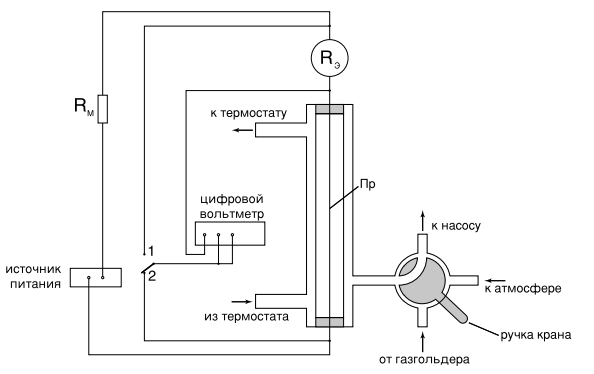
\includegraphics[width=0.55\textwidth]{setup.PNG}
    \caption{Схема экспериментальной установки}
    \label{fig:vac}
\end{figure}
Установка изготовлена из стекла и состоит из форвакуумного баллона (ФБ), высоковакуумного диффузионного насоса (ВН), высоковакуумного баллона (ВБ), масляного (М) и ионизационного (И) манометров, термопарных манометров (М1 и M2), форвакуумного насоса (ФН) и соединительных кранов
К1, К2, ..., К6 (рис. 1). Кроме того, в состав установки входят: вариатор
(автотрансформатор с регулируемым выходным напряжением), или реостат
и амперметр для регулирования тока нагревателя диффузионного насоса.
\newpage

\section{Обработка результатов измерений}
\begin{enumerate}
\item Запустим воздух в систему и подождем, пока он заполнит установку. Запустим форсвакуумный насос, чтобы он откачал воздух из установки. Давление в установке уменьшается, продолжим откачку до момента, когда $P = (2.0 \pm 0.1) \cdot 10^{-2}$ мм рт. ст. Отсоединим установку от форвауумного насоса, а затем объём, заключенный в кранах и капиллярах форвакуумной части, откроем на всю форвакуумную часть. Тогда давление изменится. Запишем высоту масла в обоих коленах маслянного манометра: 

$h_1 = (39.6 \pm 0.1)$ см масл. ст., $h_2 = (13.1 \pm 0.1)$ см масл. ст., $\Delta h_{фв} = h_1 - h_2 = (26.5 \pm 0.1)$ см масл. ст.

Плотность масла равна $\rho = 0.885$ г/см$^3$


\item Зная объём "запертого" воздуха $V_{к5+к6+кап} = 50 ~ см^3$ и используя соотношение $P_1/P_2=V_2/V_1$, вычислим объём форвауумной части установки. При этом давление $P_1 = P_{атм} = (98.8 \pm 0.1) ~ кПа$ $P_2 = \rho_{масл} g \Delta h_{фв}$. Получаем $V_{фв} = (2.17 \pm 0.01)$ л.


\item Откроем краны так, чтобы воздух, занимавший до сих пор только форсвакуумную часть установки, заполнил и высоковакуумную часть. Вновь измерим и запишем показания масляного манометра: $h_3 = (35.2 \pm 0.1)$ см масл. ст., $h_4 = (18.3 \pm 0.1)$ см масл. ст., $\Delta h_{фв} = h_3 - h_4 = (16.9 \pm 0.1)$ см масл. ст.

Рассчитаем объем высоковакуумной части: $V_{вв} = (1.23 \pm 0.02)$ л. Полный объем установки:

\begin{center}
    $V_{уст} = (3.40 \pm 0.02)$ л
\end{center}

\item Найдем скорость откачки $W$ системы по ухудшению и улучшению вакуума. Для этого открывая и закрывая кран $К_3$ будем то подключать насос к объёму, то отключать его, при этом на видео зафиксируем показания манометра от времени и построим графики (Рис. 2, Рис. 3).


\item Рассмотрим сначала улучшение вакууума.


Воспользуемся формулой
    \begin{center}
    $P - P_{пр}= (P_0 - P_{пр})\cdot exp(-\frac{W}{V}t)$.
    \end{center}
    Получим:
    \begin{center}
    $ln(P - P_{пр}) = -\frac{W}{V}t + ln(P_0 - P_{пр})$.
    \end{center}
    В координатах $ln(P - P_{пр})(t)$ построим график зависимости давления в высоковакуумной части при улучшении вакуума от времени. Коэффициент угла наклона $k = -\frac{W}{V}$. 
    
    Предельное значение достигнутого давления в системе со стороны высоковакуумной части $P_{пр} = (5.6 \pm 0.1) \cdot 10 ^{-5}$ мм рт. ст. Зная объем высоковакуумного баллона $V=1,23\pm0,02 $ и усреднив значение коэфициента наклона построенных прямых в координатах $ln(P - P_{пр})(t) $ ($k=0,219\pm0,003 л^{2}/с$) , найдем скорость откачки системы
    \begin{center}
    
     $W_1 =-kV = (2,64 \pm 0,01)\cdot 10^{-2}$ л/с
    \end{center}
  \begin{figure}[h!]
    \centering
    \includegraphics[scale=0.72]{улучшение.png}
    \caption{Зависимость давления от времени, улучшение вакуума}
\end{figure}

\begin{figure}[h!]
    \centering
    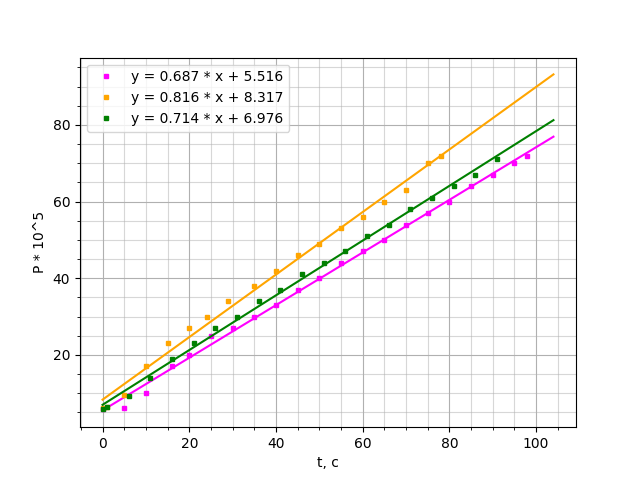
\includegraphics[scale=0.72]{ухудшение.png}
    \caption{Зависимость давления от времени, ухудшение вакуума}
\end{figure}

    
    
\item Рассмотрим ухудшение вакуума. Оценим величину потока газа $Q_Н$, поступающего из насоса назад в откачиваемую систему. Уравнения для этого имеет следующий вид: $V_vdP = (Q_Д + Q_Н) dt$ (принебрегаем при этом $Q_I$ - потоком газа, образующимся за счет течи в системе).



Построим графики зависимости $P(t)$ и определим для них коэффициенты угла наклона прямой. Усредненное значение угла наклона $ k=(0,74 \pm 0,01) \cdot 10^{-5}~торр/с$. Тогда получим $(Q_Д + Q_Н) = kV_v = (0,91 \pm 0,02) \cdot 10^{-5} ~торр \cdot л/c $


Вследствие того, что $Q_\text{Д}$ обычно порядка $10^{-8}$, то  считаем $Q_\text{Н} + Q_\text{Д} \approx Q_\text{Н}$. Таким образом,
	$$Q_\text{Н} = (9,1 \pm 0,2)\cdot 10^{-6} ~\text{торр}\cdot\text{л/c}$$
	\item
	Рассчитаем производительность насоса ещё одним способом: создав искусственную течь. Открываем кран $K_6$ при включённом  насосе и измеряем давление, установившееся при течи. Оно равно $$P_\text{уст} = (1,0\pm 0,1) \cdot 10^{-4} ~\text{торр}.$$
	Запишем (10) для данного случая:
		$$P_\text{пр}W = Q_1, \quad P_\text{уст}W = Q_1 + \frac{d(PV)_\text{капилляр}}{dt}$$
	С учётом (7) получаем:
	$$(P_\text{уст} - P_\text{пр})W = \frac{4}{3}(d/2)^3\sqrt{\frac{2\pi RT}{\mu}}\frac{P_\text{фв}}{L},$$
	где d и L --- диаметр и длина капилляра, равные
	$$d = 0,8\pm 0,1 ~\text{мм},\quad L = 10,8\pm 0,1 ~\text{cм}$$
	Получаем:
	$$W_2 = (1,5\pm 0,8) \cdot 10^{-2} ~\text{л/c}$$
\end{enumerate}
Сравним полученное нами значение скорости откачки с значением из пункта 5:

\begin{center}
$W_1 = (2,6 \pm 0,1) \cdot 10^{-2}$ л/с\\
$W_2 = (1,5 \pm 0,8) \cdot 10^{-2}$ л/с
\end{center}

\section{Выводы}

В ходе данной работы было проведено ознакомление с вакуумной техникой.

\begin{enumerate}

\item Были измерены объемы форсвакуумной части, высоковакуумной и объем всей установки: $V_{фв} = (2.17 \pm 0.01)$ л,  $V_{вв} = (1.23 \pm 0.02)$ л, $V_{уст} = (3.40 \pm 0.02)$ л. 

\item Двумя способами была определена скорость откачки диффузионного насоса: по улучшению вакуума и по разности давлений при впускании в высоковакуумную часть искусственной течи и предельного давления в высоковакуумной части установки. Полученные результаты:
\begin{center}
$W_1 = (2,6 \pm 0,1) \cdot 10^{-2}$ л/с\\
$W_2 = (1,5 \pm 0,8) \cdot 10^{-2}$ л/с
\end{center}

Полученные нами значения плохо совпадают в пределах погрешностей.  Основная предполагаемая причина несовпадения результатов заключается в том, что в формуле для определения скорости откачки вторым способом фигурирует температура. Для расчета была взята комнатная температура, но температура воздуха в установке по факту выше: его нагревают элементы, нагревающие масло в диффузионном насосе. Эта температура достаточно велика, поэтому конечное значение скорости откачки, определяемое вторым способом, должно быть несколько выше полученного нами значения.

\item Определён поток воздуха, вытекающий через насос назад в высоковакуумную часть установки при откачке:
	$$Q_\text{Н} = (9,1 \pm 0,2)\cdot 10^{-6} ~\text{торр}\cdot\text{л/c}$$
 Эта величина оказалась сравнительно мала (на 4 порядка меньше) по сравнению с определённой экспериментально двумя способами скоростью откачки насоса.



\end{enumerate}

\end{document}
